%-------------------------------------------------------%
\section{Creating the initial and boundary data: init} \label{sec:tutorial_real_init}
%-------------------------------------------------------%

Move to the directory \verb|init| and create the initial and boundary data for the \scalerm simulation as follows:
\begin{verbatim}
 $ cd ${Tutorial_DIR}/real/experiment/init
 $ ls
    init.d01.conf
    init.launch.conf
    param.bucket.conf
    scale-rm_init
\end{verbatim}

In the directory \verb|init|, there exists the configuration file \verb|init.d01.conf|.
The file \verb|init.launch.conf| also exists but is not used here.
It is necessary to edit the file \verb|init.d01.conf| according to such experimental settings as \verb|pp.d01.conf|. \verb|init.d01.conf| has been already edited for this tutorial experiment as shown in Table \ref{tab:grids}.  To create the initial and boundary data,  the topographical data generated in the previous section is used. This is set in \verb|init.d01.conf| to refer the relative path as follows:

\editbox{
\verb|&PARAM_TOPOGRAPHY| \\
\verb|   TOPOGRAPHY_IN_BASENAME = "../pp/topo_d01",| \\
\verb|/| \\
 \\
\verb|&PARAM_LANDUSE| \\
\verb|   LANDUSE_IN_BASENAME = "../pp/landuse_d01",| \\
\verb|/| \\
}
In particular,  the contents of \namelist{PARAM_MKINIT_REAL_ATMOS}, \namelist{PARAM_MKINIT_REAL_OCEAN} and \namelist{PARAM_MKINIT_REAL_LAND} are handled. It should be confirmed that the settings in \verb|init.d01.conf| are correct.
\editboxtwo{
\verb|&PARAM_MKINIT_REAL_ATMOS| & \\
\verb| NUMBER_OF_FILES      = 2,|                                   & {\small : number of files read } \\
\verb| FILETYPE_ORG         = "GrADS",|                             & {\small : choose from Table \ref{tab:inputdata_format}} \\
\multicolumn{2}{l}{\verb| BASENAME_ORG        = "namelist.grads_boundary.FNL.2005053112-2015011400",|}     \\
\verb| BASENAME_BOUNDARY    = "boundary_d01",|                      & {\small : output name of boundary data} \\
\verb| BOUNDARY_UPDATE_DT   = 21600.0,|                             & {\small : time interval of input data} \\
\verb| PARENT_MP_TYPE       = 3,|                                   & \\
\verb| USE_FILE_DENSITY     = .false.,|                             & {\small : use the atmospheric density in the parent model or not?} \\
\verb|/| \\
\\
\verb|&PARAM_MKINIT_REAL_OCEAN| & \\
\verb|   .........              |  & \\
\verb| INTRP_OCEAN_SFC_TEMP = "mask",|                              & {\small : how to treat the missing value of SST} \\
\verb| INTRP_OCEAN_TEMP     = "mask",|                              & {\small : how to treat the missing value of SST} \\
\verb|/| \\
\\
\verb|&PARAM_MKINIT_REAL_LAND| & \\
\verb|   ..........              | & \\
\verb| USE_FILE_LANDWATER   = .true.,|                              & {\small : use soil moisture data in the parent model or not?} \\
\verb| INTRP_LAND_TEMP      = "mask",|                              & {\small : how to treat the missing value of soil temperature} \\
\verb| INTRP_LAND_WATER     = "fill",|                              & {\small : how to treat the missing value of soil moisture} \\
\verb| INTRP_LAND_SFC_TEMP  = "fill",|                              & {\small : how to treat the missing value of surface temperate} \\
\verb|/| \\
}

The file format of the meteorological field data is specified in \nmitem{FILETYPE_ORG}. In this case, it is given as ``\grads'' to read data in \grads format. Refer to Section \ref{sec:adv_datainput} for the details of the input file.


Link the input data (FNL) that are converted into binary form in Section \ref{sec:tutorial_real_data} to the current working directory. A shell script for this appropriate linkage is prepared as \verb|"gradsinput-link_FNL.sh"| in the directory \verb|${Tutorial_DIR}/real/data|:
\begin{verbatim}
  $ cp ../../data/gradsinput-link_FNL.sh ./
  $ sh gradsinput-link_FNL.sh
\end{verbatim}
If the following linkages are found, it is successfully concluded.
\msgbox{
\verb|ATM_00000.grd -> ../tools/FNL_output/200707/FNL_ATM_2007071418.grd| \\
\verb|ATM_00001.grd -> ../tools/FNL_output/200707/FNL_ATM_2007071500.grd| \\
\verb|LND_00000.grd -> ../tools/FNL_output/200707/FNL_LND_2007071418.grd| \\
\verb|LND_00001.grd -> ../tools/FNL_output/200707/FNL_LND_2007071500.grd| \\
\verb|SFC_00000.grd -> ../tools/FNL_output/200707/FNL_SFC_2007071418.grd| \\
\verb|SFC_00001.grd -> ../tools/FNL_output/200707/FNL_SFC_2007071500.grd| \\
}

Then, link a namelist file to the directory \verb|init| to read the binary (\grads) data format in SCALE.
\begin{verbatim}
  $ ln -s ../../data/namelist.grads_boundary.FNL.2005053112-2015011400 ./
\end{verbatim}
After the above preparations, execute the \verb|scale-rm_init| using four MPI processes.
\begin{verbatim}
 $ mpirun -n 4 ./scale-rm_init init.d01.conf
\end{verbatim}

If the job finishes normally, the following files are generated:
\begin{verbatim}
 $ ls
    boundary_d01.pe000000.nc
    boundary_d01.pe000001.nc
    boundary_d01.pe000002.nc
    boundary_d01.pe000003.nc
    init_d01_20070714-180000.000.pe000000.nc
    init_d01_20070714-180000.000.pe000001.nc
    init_d01_20070714-180000.000.pe000002.nc
    init_d01_20070714-180000.000.pe000003.nc
    init_LOG_d01.pe000000
\end{verbatim}
The file \verb|init_LOG_d01.pe000000| is a log file.  The following message is output at the end of the file \verb|init_LOG_d01.pe000000|:
\msgbox{
 +++++ Closing LOG file\\
}
The file sizes of the boundary and initial data, \verb|boundary_d01.pe######.nc| and \\
\verb|init_d01_20070714-180000.000.pe######.nc|, are approximately 18.9 MB and 12.6 MB, respectively,  where \verb|######| represents the MPI process number.\\

\vspace{0.8cm}
\noindent {\Large\em NOTICE}: {\large Reduction of memory usage when reading input data} \hrulefill

In \scalerm, only the master process reads input data and broadcasts the data to each node.
This algorithm can reduce file I/O and process the input data fast.
On the other hand, the algorithm may cause insufficient memory error when reading large input data, especially on a high-performance computing system.
To avoid the error, you can choose the method that each node reads input data by itself.
%
\editboxtwo{
\verb|&PARAM_MKINIT_REAL_ATMOS| & \\
\verb| SERIAL_PROC_READ = .false.,| & {\small : Does only the master process read input data?} \\
\verb|/| \\
}
%
The default setting is \verb|.true.|, which means that the master process only reads input data.
When setting \verb|.false.|, each node accesses to only the data it needs, resulting in the reduction of memory usage.
However, because the algorithm places a load on file I/O,
the computational performance may deteriorate due to locking file access.

\noindent \hrulefill\\

\vspace{0.8cm}
\noindent {\Large\em OPTION} \hrulefill \\
When ``gpview'' is installed,  one can confirm whether the initial and boundary data have been created correctly  by the following command:
\begin{verbatim}
 $ gpvect --wsn=1 --scalar --slice z=1500 --nocont --aspect=1 --range=0.002:0.016         \
          --int 0.001 --xintv=10 --yintv=10 --unit_vect                                   \
          init_d01_20070714-180000.000.pe00*@QV  init_d01_20070714-180000.000.pe00*@MOMX  \
          init_d01_20070714-180000.000.pe00*@MOMY --title "QV, MOMX, MOMY"
\end{verbatim}
If the same figure as Fig. \ref{fig:init} is found, it is successfully concluded.

\begin{figure}[h]
\begin{center}
  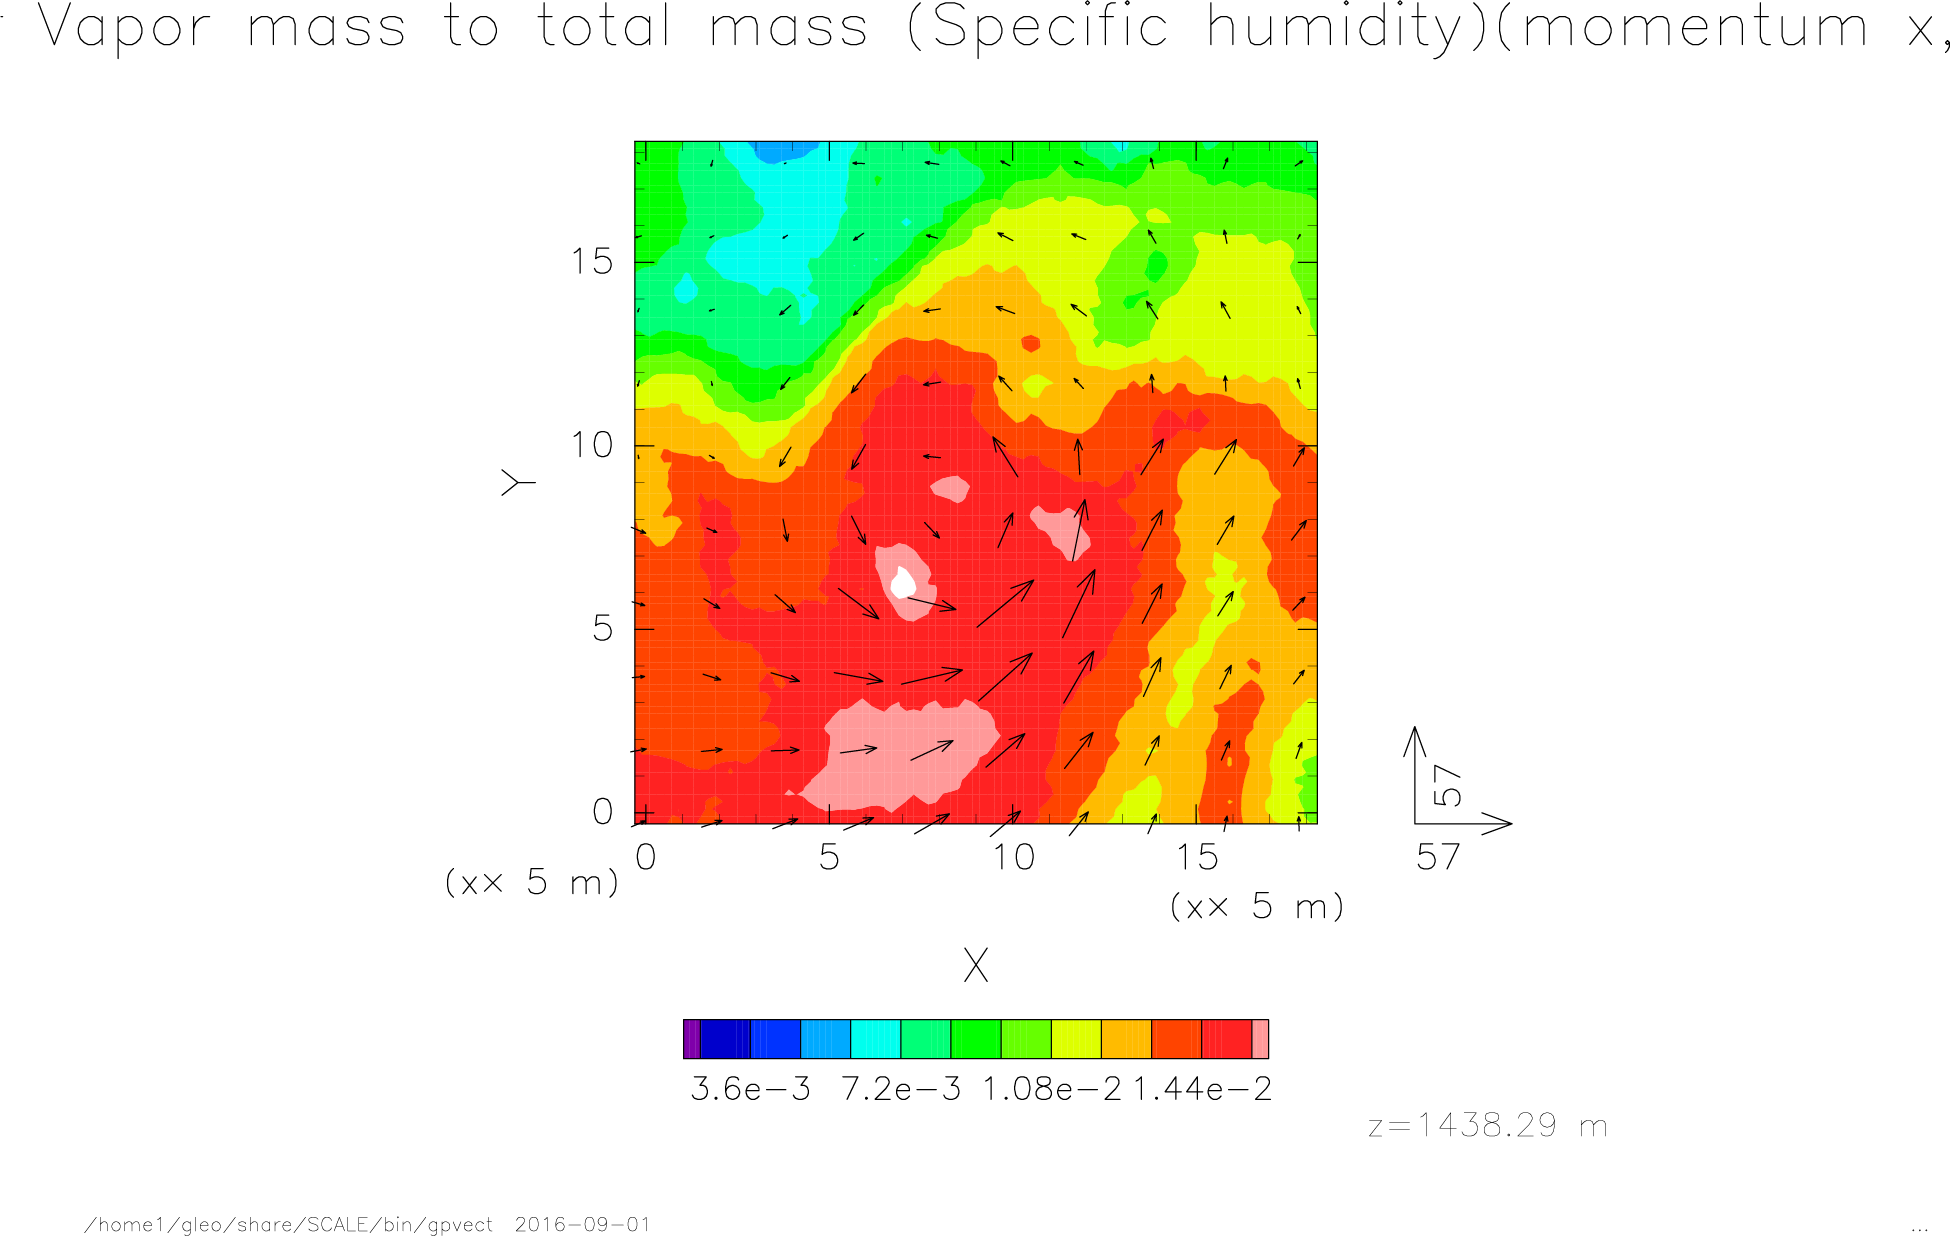
\includegraphics[width=0.6\hsize]{./../../figure/real_init_qv-momxy.pdf}\\
  \caption{Initial field at z=1500m for the tutorial experiment.
    The color indicates specific humidity and the vector horizontal momentum flux.}
  \label{fig:init}
\end{center}
\end{figure}
